\documentclass[zihao=false,fontset=windows]{ctexart}
% ctexart 不接受任意 pt 选项。正文改 {9.5pt}，方括号里是对应行距。
\usepackage{scrextend}
\changefontsizes[12pt]{10pt}

\usepackage[a4paper,left=2.35cm,right=2.35cm,top=1.7cm,bottom=1.9cm]{geometry}
\usepackage{xcolor}
\usepackage{graphicx}
\usepackage{amsmath,amssymb}
\usepackage{enumitem}
\usepackage{tabularx}
\usepackage{colortbl}
\usepackage{listings}
\usepackage{hyperref}
\usepackage[most]{tcolorbox}

\definecolor{feishuText}{RGB}{31,35,41}
\definecolor{feishuBlue}{RGB}{36,91,219}
\definecolor{feishuRed}{RGB}{216,57,49}
\definecolor{feishuGray}{RGB}{100,106,115}
\definecolor{feishuGray2}{RGB}{143,149,158}
\definecolor{feishuPinkBg}{RGB}{251,191,188}
\definecolor{quoteBar}{RGB}{51,112,255}
\definecolor{codebg}{RGB}{245,246,247}
\definecolor{codeborder}{RGB}{222,224,227}
\definecolor{inlinebg}{RGB}{242,243,245}
\definecolor{callRed}{RGB}{253,226,226}
\definecolor{callOrange}{RGB}{255,245,235}
\definecolor{callYellow}{RGB}{254,255,240}
\definecolor{callGreen}{RGB}{240,251,239}
\definecolor{callBlue}{RGB}{240,244,255}
\definecolor{callRedSoft}{RGB}{254,241,241}
\definecolor{callSun}{RGB}{255,255,204}
\definecolor{tableHead}{RGB}{242,243,245}
\definecolor{tableRule}{RGB}{222,224,227}
\definecolor{codeText}{RGB}{31,35,41}
\definecolor{codeKeyword}{RGB}{0,0,255}
\definecolor{codeComment}{RGB}{0,128,0}
\definecolor{codeString}{RGB}{163,21,21}

\setmainfont{Times New Roman}
\setCJKmainfont{Microsoft YaHei}[AutoFakeBold=2.2]
\setCJKsansfont{Microsoft YaHei}[AutoFakeBold=2.2]
\setCJKmonofont{Microsoft YaHei}[AutoFakeBold=2.2]
\setmonofont{Consolas}
\newfontfamily\emojifont{Segoe UI Emoji}

\hypersetup{
  colorlinks=true,
  urlcolor=feishuBlue,
  linkcolor=feishuBlue,
  unicode=true,
  pdftitle={ALBEF(2021, Salesforce Research)}
}

\setlength{\parindent}{0pt}
\setlength{\parskip}{0.42em}
\setlength{\fboxsep}{1.5pt}
\setlength{\emergencystretch}{3em}
\linespread{1.28}
\color{feishuText}
\arrayrulecolor{tableRule}
\urlstyle{same}

\setlist[enumerate]{label=\textcolor{feishuBlue}{\arabic*.}, leftmargin=1.7em, itemsep=0.22em, topsep=0.28em, parsep=0.08em, partopsep=0pt}
\setlist[itemize,1]{label=\textcolor{feishuBlue}{\textbullet}, leftmargin=1.35em, itemsep=0.18em, topsep=0.25em, parsep=0.06em, partopsep=0pt}
\setlist[itemize,2]{label=\textcolor{feishuBlue}{◦}, leftmargin=1.45em, itemsep=0.12em, topsep=0.15em}
\setlist[itemize,3]{label=\textcolor{feishuBlue}{\rule[0.18em]{0.38em}{0.38em}}, leftmargin=1.55em, itemsep=0.1em, topsep=0.12em}

\newcommand{\feiEmoji}[1]{{\emojifont #1}}
\newcommand{\incode}[1]{\colorbox{inlinebg}{\ttfamily\small #1}}
\newcommand{\bigmath}[1]{%
  \begin{center}\large$\displaystyle #1$\end{center}%
}

\lstset{
  language=Python,
  basicstyle=\ttfamily\footnotesize\color{codeText},
  keywordstyle=\color{codeKeyword},
  commentstyle=\color{codeComment},
  stringstyle=\color{codeString},
  showstringspaces=false,
  breaklines=true,
  columns=fullflexible,
  keepspaces=true,
  tabsize=4,
  upquote=true,
  aboveskip=2pt,
  belowskip=0pt,
  xleftmargin=0pt,
  frame=none
}

\tcbset{
  feishubase/.style 2 args={
    enhanced,
    boxrule=0pt,
    arc=8pt,
    left=10pt,
    right=10pt,
    top=7pt,
    bottom=7pt,
    before skip=6pt,
    after skip=6pt,
    colback=#1,
    colframe=#1,
    before upper={\feiEmoji{#2}\hspace{0.45em}\ignorespaces}
  }
}
\newtcolorbox{feishubox}[2]{feishubase={#1}{#2}, breakable}
\newtcolorbox{feishuboxnb}[2]{feishubase={#1}{#2}}

\newtcolorbox{feishuquote}{
  enhanced,
  breakable,
  boxrule=0pt,
  leftrule=3pt,
  arc=0pt,
  colframe=quoteBar,
  colback=white,
  left=8pt,
  right=2pt,
  top=2pt,
  bottom=2pt,
  before skip=4pt,
  after skip=4pt,
  before upper=\color{feishuGray}
}

\newtcolorbox{feishucode}{
  enhanced,
  breakable,
  colback=codebg,
  colframe=codeborder,
  boxrule=0.6pt,
  arc=6pt,
  left=6pt,
  right=6pt,
  top=5pt,
  bottom=4pt,
  before skip=6pt,
  after skip=6pt
}

\begin{document}
{\zihao{1}\bfseries ALBEF(2021, Salesforce Research)\par}
\vspace{0.15em}

\begin{feishuquote}
ALBEF：对齐图文单模态表征（2021，Salesforce Research）\par
\href{https://arxiv.org/abs/2107.07651}{ALign BEfore Fuse}\par
\end{feishuquote}
\vspace{0.45em}
\textbf{视觉语言预训练（Vision-and-Language Pre-training，VLP）}的目标是从大规模 image-text 对中学习多模态的表示，用于改善下游的视觉语言任务（Vision-and-Language，V+L）。\par
\vspace{0.45em}
主流VLP模型分类两种：\par
\begin{tcbraster}[raster columns=2, raster equal height=rows, raster column skip=9pt, raster row skip=8pt, raster left skip=0pt, raster right skip=0pt]
\begin{feishuboxnb}{callRed}{🌟}
\textbf{双塔结构 (Dual Encoder)}：\par
图像有一个Encoder建模视觉信息，文本有一个Encoder建模文本信息，双塔完全分开，互不干扰，模态之间的交互用非常简单的余弦相似度来完成。\par
\textcolor{feishuBlue}{优点：对检索任务很有效，时间复杂度为线性}\par
\textcolor{feishuBlue}{缺点：模态交互部分太过简单，浅层的交互不足以处理复杂的 VL 分类任务}\par
\end{feishuboxnb}
\begin{feishuboxnb}{callRed}{🌟}
\textbf{单塔结构 (Fusion Encoder)}：\par
Fusion Encoder的方式，先把图像和文本分开处理，然后在做模态交互的时候，用一个Transformer Encoder做模态之间的交互。\par
\textcolor{feishuBlue}{优点：弥补双塔模式的缺陷，在VR、VE、VQA任务上效果很好}\par
\textcolor{feishuBlue}{缺点：推理速度慢（在处理检索任务的时候，需要联合编码所有可能的图像-文本对来计算检索任务的相似度分数，二次时间复杂度导致推理速度比双塔结构慢得多）}\par
\end{feishuboxnb}
\end{tcbraster}
\vspace{0.45em}
在多模态模型发展最初的时候，大部分模型存在三大局限：\par
\begin{tcbraster}[raster columns=3, raster equal height=rows, raster column skip=9pt, raster row skip=8pt, raster left skip=0pt, raster right skip=0pt]
\begin{feishuboxnb}{callOrange}{📝}
\textbf{缺乏细粒度跨模态交互}：\par
仅学习单模态编码器，难以建模图像与文本的复杂关系，限制了细粒度理解能力。\par
\end{feishuboxnb}
\begin{feishuboxnb}{callOrange}{📝}
\textbf{多模态融合存在不对齐问题}：\par
在输入多模态融合模型之前，如果图像特征和文本特征未对齐，那么跨模态对齐很难学习。\par
\end{feishuboxnb}
\begin{feishuboxnb}{callOrange}{📝}
\textbf{预训练数据噪声影响学习}：\par
主流 VLP 模型依赖从互联网收集的噪声图文对，但MLM等训练目标易过拟合噪声文本，影响表示学习质量。\par
\end{feishuboxnb}
\end{tcbraster}
那什么样的多模态架构效果会比较好呢？\par
在ViLT论文中，多模态架构根据编码层、交互层的强弱分为了四种框架：\par
\begin{center}
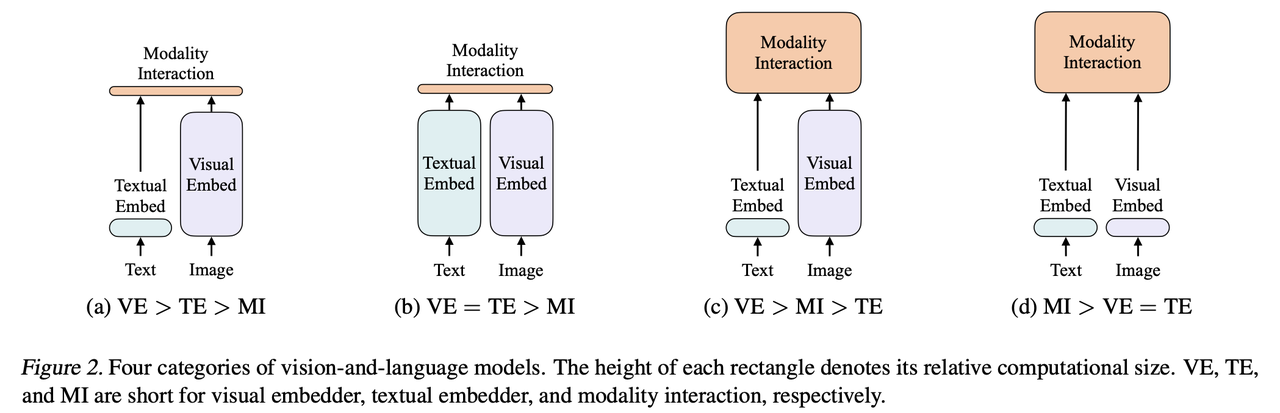
\includegraphics[width=0.980\textwidth]{images/2021-NeurIPS-ALBEF/fig-675.png}
\end{center}
\begin{tcbraster}[raster columns=2, raster equal height=rows, raster column skip=9pt, raster row skip=8pt, raster left skip=0pt, raster right skip=0pt]
\begin{feishuboxnb}{callYellow}{🛖}
a是VSE/VSE++的架构：\par
文本端直接抽一个文本特征；\par
视觉端非常大，是一个目标检测器，基于Bouding Box的视觉特征；\par
非常简单的模态之间的交互。\par
\end{feishuboxnb}
\begin{feishuboxnb}{callOrange}{🛖}
b是CLIP的架构：\par
文本端和视觉端采用同等复杂程度的encoder进行特征提取；\par
简单的模态交互（点乘）。\par
\end{feishuboxnb}
\end{tcbraster}
\begin{tcbraster}[raster columns=2, raster equal height=rows, raster column skip=9pt, raster row skip=8pt, raster left skip=0pt, raster right skip=0pt]
\begin{feishuboxnb}{callGreen}{🛖}
c是Oscar或者ViLBERT、Uniter等采用的架构：\par
文本端很简单，视觉端非常大；\par
更复杂的模态之间的交互（Transformer的Encoder或是其他复杂模型）。\par
\end{feishuboxnb}
\begin{feishuboxnb}{callBlue}{🛖}
d是ViLT的架构；\par
文本端和视觉端都非常简单，视觉端参考ViT论文，直接使用一层Patch Embedding提取特征，基于Patch的视觉特征；\par
更复杂的模态之间的交互（Transformer的Encoder或是其他复杂模型）。\par
\end{feishuboxnb}
\end{tcbraster}
这些架构对模型的选择和loss函数的选择都有启发：\par
\begin{tcbraster}[raster columns=2, raster equal height=rows, raster column skip=9pt, raster row skip=8pt, raster left skip=0pt, raster right skip=0pt]
\begin{feishuboxnb}{callRedSoft}{✨}
模型的结构选择：\par
\begin{enumerate}
\item 有两个分支分别抽取图像-文本特征；
\item 视觉特征重要性大于文本特征，需要使用更强的视觉特征；
\item 多模态融合的模型要尽可能大。
\end{enumerate}
\end{feishuboxnb}
\begin{feishuboxnb}{callRedSoft}{✨}
loss的选择：\par
\begin{enumerate}
\item Image Text Contrastive Loss（ITC）：CLIP中使用的对比学习的ITC的loss训练，效果好且训练高效；
\item Image Text Matching Loss（ITM）：在c和d中都有使用，且效果较好；
\item Mask Language Modeling（MLM）：BERT的训练方式，NLP和CV中都统一用的训练方式。
\end{enumerate}
（以上这些loss在ALBEF中有详细介绍）\par
\end{feishuboxnb}
\end{tcbraster}
\vspace{0.45em}
\par\vspace{1.15em}\noindent{\zihao{-2}\bfseries ALBEF 概述}\par\vspace{0.28em}
ALBEF主要针对两种现有问题提出了两种贡献：\par
\begin{enumerate}
\item 针对\textcolor{feishuBlue}{现有方法采用基于Transformer的多模态编码器，联合编码图片特征和文本特征，未将两者对齐}的问题，ALBEF采用了模态融合前先对齐（Align Before Fusion）的方法来解决对齐问题，分别使用各自的encoder对image-text进行独立编码，然后使用多模态encoder通过cross attention将image特征和text特征进行融合。
\item 针对\textcolor{feishuBlue}{image-text数据集是从Web上收集的，内容比较嘈杂，存在噪声}的问题，ALBEF提出了动量蒸馏（Momentum Distillation，MoD）的方法来解决网络脏数据问题，训练时通过模型参数的移动平均保留一个动量版本的模型，然后使用动量模型生成伪标签作为额外的监督信号。使用MoD后，模型不会因为产生与网络注释不同的其他合理输出而受到惩罚。
\end{enumerate}
\vspace{0.45em}
ALBEF的\textcolor{feishuRed}{\textbf{核心方法}}：\par
\begin{enumerate}
\item 使用无检测器图像编码器和文本编码器对图像和文本进行独立编码；
\item 使用图像-文本对比损失（ITC loss）对图文特征进行对齐； 
\item 使用多模态编码器通过跨模态注意将图像特征与文本特征融合。
\end{enumerate}
从互信息最大化角度理解ALBEF：\par
ITC 和 MLM 最大化了图像-文本对的不同视图之间的互信息下限，其中视图是通过从每个视图对中获取部分信息生成的。从这个角度来看，动量蒸馏可以解释为利用语义相似的样本生成新的视图。因此，ALBEF 可学习不受语义保留变换影响的视觉语言表征。\par
\par\vspace{1.15em}\noindent{\zihao{-2}\bfseries 预训练}\par\vspace{0.28em}
\par\vspace{0.95em}\noindent{\zihao{3}\bfseries 2.1 模型结构}\par\vspace{0.28em}
\begin{center}
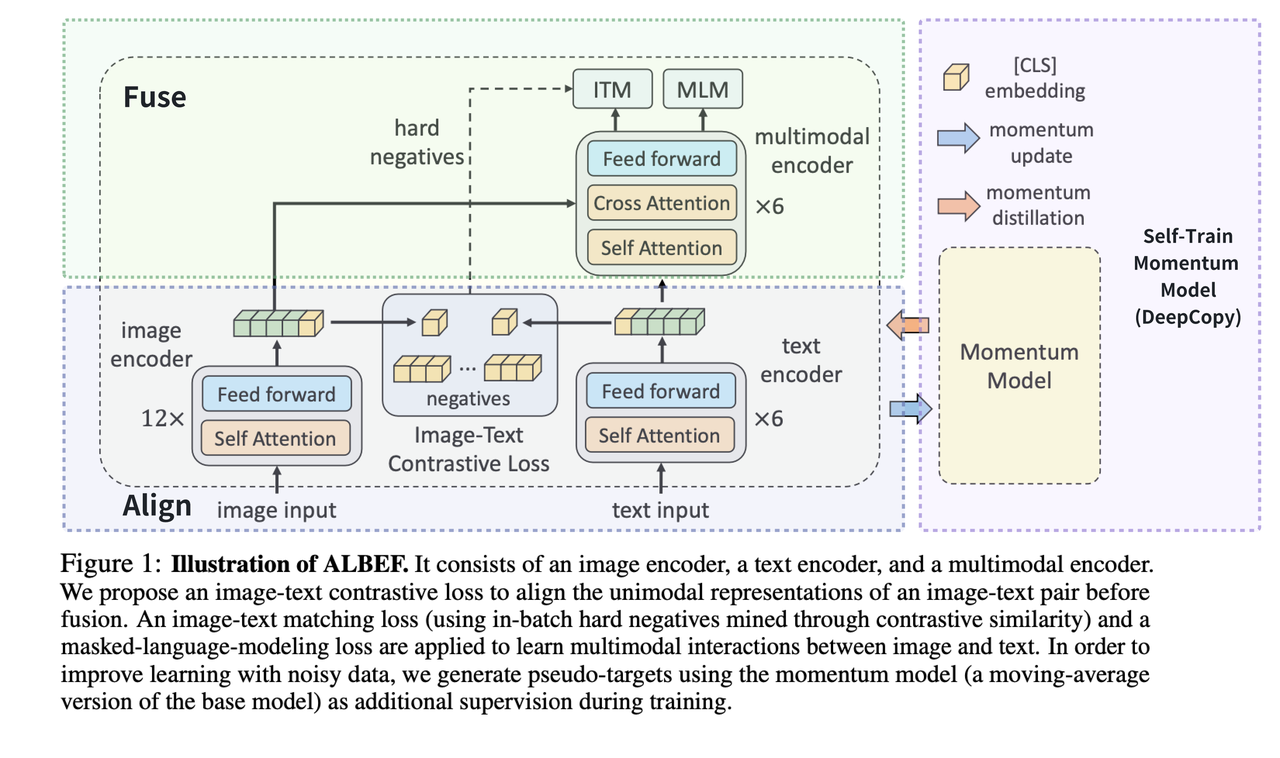
\includegraphics[width=0.980\textwidth]{images/2021-NeurIPS-ALBEF/fig-728.png}
\end{center}
如上图所示，ALBEF包含：\textcolor{feishuRed}{1个图像编码器}、\textcolor{feishuRed}{1个文本编码器}、\textcolor{feishuRed}{1个多模态编码器}和\textcolor{feishuRed}{1个同样包含上述3个编码器的动量(教师)模型}。\par
对齐（Align）阶段包含图像编码器和文本编码器，类似于CLIP；融合（Fuse）阶段使用cross attention作为token mixer；动量蒸馏模型的初始化由原始的三个模型拷贝而来，与原始模型结构完全一样。\par
\par\vspace{0.75em}\noindent{\zihao{4}\bfseries 2.1.1 图像编码器}\par\vspace{0.28em}
ALBEF的图像编码器使用\textcolor{feishuRed}{\textbf{12层}}的 ViT-B/16，然后使用在 ImageNet-1K 上预训练得到的权重来进行初始化。按照 \href{https://scnajei2ds6y.feishu.cn/wiki/QEJ8wXq9GiTBrxkMqbScnd8nnod}{ViT} 的做法，会先将输入图像打成 patch，然后通过 patch embedding 输入到 ViT encoder 中进行注意力的学习，输入图像被编码后的序列表示为${v_{cls},v_1,...,v_N}$，其中$v_{cls}$是\incode{[cls]}的Embedding向量（图中黄色格子），它代表了图像特征的全局表达。\par
\par\vspace{0.75em}\noindent{\zihao{4}\bfseries 2.1.2 文本编码器}\par\vspace{0.28em}
ALBEF的文本编码器使用\textcolor{feishuRed}{\textbf{6层}}的Transformer Encoder，用$BERT_{base}$的前6层进行初始化，输入文本$T$的Embedding输出序列表示为${w_{cls},w_1,...,w_N}$，其中$w_{cls}$也是\incode{[cls]}token（图中黄色格子），它代表了整个句子的文本信息。\par
\par\vspace{0.75em}\noindent{\zihao{4}\bfseries 2.1.3 多模态编码器}\par\vspace{0.28em}
ALBEF的多模态编码器使用\textcolor{feishuRed}{\textbf{6层}}的Transformer Encoder（含cross attention），使用$BERT_{base}$的后6层进行初始化（BERT不包含cross attention，所以这里面的cross attention是随机初始化的），将图像特征向量和文本特征向量输入到多模态编码器中，通过每层的\textcolor{feishuRed}{\textbf{cross attention}}将图像特征和文本特征进行融合，输入是图像编码器和文本编码器输出的向量，输出是融合向量（可以理解为\textcolor{feishuBlue}{以图像向量为指导经过6个含cross attention的transformer模块优化过的文本向量}），然后就可以执行下游的两个任务：\textbf{图文匹配ITM}、\textbf{掩码学习MLM}。\par
\par\vspace{0.75em}\noindent{\zihao{4}\bfseries 2.1.4 动量模型}\par\vspace{0.28em}
ALBEF的动量模型是额外保存的一个模型，同样包括图像编码器、文本编码器、多模态编码器，且初始化参数也一致（借助动量编码器MoCo的思想，完全copy左边的模型，也可以称作教师模型）。但动量模型不通过梯度优化，而是用左边训练好的模型参数通过\textbf{EMA（指数移动平均）}进行参数更新。然后根据动量模型的\textbf{soft target}来将知识蒸馏到学生模型，以此来减弱噪音数据对主干模型的影响。\par
\begin{feishuquote}
梯度模型：正常通过梯度优化更新参数的模型，左边的模型\par
动量模型：额外保存的通过指数移动平均更新参数的模型\par
指数移动平均EMA的公式可表达为$\theta_t=\lambda \theta_t + (1-\lambda)\theta_g$，其中$\theta_t$和$\theta_g$分别为动量模型和梯度模型的参数，$\lambda$（moving average）设置的很大，论文中为0.995，目的：动量模型不会那么快更新，产生的特征更加稳定，保证动量模型的稳定使其不会因为噪声干扰而偏离原本正确的优化方向，那么这样的话不仅可以做更稳定的负样本采样，而且还可以去做动量蒸馏。\par
\end{feishuquote}
\par\vspace{0.75em}\noindent{\zihao{4}\bfseries 补充}\par\vspace{0.28em}
为什么ALBEF要选择12层ViT作为图像编码器、6层Transformer作为文本编码器、6层Transformer作为多模态编码器这种架构？\par
\begin{feishubox}{callRedSoft}{✨}
从最前面介绍的4种多模态架构图中，可以总结出，想要得到一个好的多模态模型，图像编码器要足够大，同时多模态编码器也要大，文本编码器不需要特别大。\par
\end{feishubox}
总结ALBEF 模型的特点：\par
\begin{enumerate}
\item 图像编码器就是 ViT，初始化权重也是来自它。
\item 文本编码器是 BERT 的一半，前6层做文本编码，初始化权重也是来自它。
\item 图像编码器的体量大于文本，经验发现这样做效果好。
\item 多模态编码器是 BERT 的另一半，后6层做多模态编码。
\end{enumerate}
\par\vspace{0.95em}\noindent{\zihao{3}\bfseries 2.2 预训练目标}\par\vspace{0.28em}
ALBEF 的预训练目标为3个：\par
\begin{enumerate}
\item 单模态编码器上的图文对比学习（\textbf{Image-Text Contrastive Learning，ITC}）
\item 多模态编码器的完形填空（\textbf{Masked Language Modeling，MLM}）
\item 图文匹配（\textbf{Image-Text Matching，ITM}）
\end{enumerate}
\par\vspace{0.75em}\noindent{\zihao{4}\bfseries 2.2.1 ITC}\par\vspace{0.28em}
ITC（Image-Text Contrastive Learning）其实就是CLIP中使用的对比学习的方法，解决图像特征与文本特征的对齐问题，其目标是在多模态交叉融合之前更好的学习单模态的表征，就是“ALign BEfore Fuse”中的\textcolor{feishuRed}{ALign}。\par
在ITC中，直接获取图像编码器和文本编码器输出向量中各自的\incode{[cls]}token作为各自的全局表征信息，然后通过线性变化映射到低维的向量空间（768变到256维），分别记为$g_v$和$g_w$。\par
ITC学习一个相似函数$s=g_v(v_{cls})^T g_w(w_{cls})$，计算两个单模态特征向量之间的相似度。通过训练使配对的图文特征相似度越来越高，不配对的图文相似度越来越低。\par
ALBEF在ITC任务中使用动量蒸馏 Momentum Distillation 来解决\textbf{图文对有噪音的问题}。在训练阶段，它会通过 moving average 的方式对每个 encoder 进行备份，备份的 encoder 输出表示为$g'_v(v'_{cls})$和$g'_w(w'_{cls})$，然后计算\textbf{和当前图像最相似的文本（image-to-text）}、\textbf{和当前文本最相似的图像（text-to-image）}作为伪目标pseudo-targets，相似度定义如下：\par
$s(I,T)=g_v(v_{cls})^T g'_w(w'_{cls})$，$s(T,I)=g_w(w_{cls})^T g'_v(v'_{cls})$\par
对于每个图像和文本，计算\incode{image-to-text}和\incode{text-to-image}的归一化相似度如下：\par
\bigmath{
p_{m}^{\mathrm{i2t}}(I)=\frac{\exp\bigl(s(I,T_{m})/\tau\bigr)}{\sum_{m=1}^{M}\exp\bigl(s(I,T_{m})/\tau\bigr)},
\quad
p_{m}^{\mathrm{t2i}}(T)=\frac{\exp\bigl(s(T,I_{m})/\tau\bigr)}{\sum_{m=1}^{M}\exp\bigl(s(T,I_{m})/\tau\bigr)}
}
注意其中的$\tau$是可以学习的温度参数，用来控制 Softmax 分布的形状。\par
\begin{feishuquote}
较小的$\tau$使得 Softmax 输出接近 one-hot，使模型更极端地关注最高相似度的样本，梯度更大，收敛更快，但可能导致过拟合；\par
较大的$\tau$使得 Softmax 输出更平滑，让模型在多个可能的匹配上进行学习，有助于泛化。\par
\end{feishuquote}
真实的one-hot相似度是$y^{i2t}(I)$和$y^{i2t}(T)$（$I$与队列中哪个$T$对应，对应位置就应该为1，其余为0），负样本对的概率为0，正样本对的概率为1。\par
所以image-text对的对比loss是$p$和$y$二者的交叉熵$H$：\par
\bigmath{
\mathcal{L}_{\mathrm{itc}}=\frac{1}{2}\mathbb{E}_{(I,T)\sim D}\Bigl[\mathrm{H}\bigl(\mathbf{y}^{\mathrm{i2t}}(I),\mathbf{p}^{\mathrm{i2t}}(I)\bigr)+\mathrm{H}\bigl(\mathbf{y}^{\mathrm{t2i}}(T),\mathbf{p}^{\mathrm{t2i}}(T)\bigr)\Bigr]
}
ITC loss（图像文本对比损失）的作用：\par
\begin{enumerate}
\item 使图像特征和文本特征一致，使多模态编码器更容易进行跨模态学习；
\item 改进单模态编码器，使其更好地理解图像和文本的语义；
\item 学习一个共同的低维空间来嵌入图像和文本，这使图像-文本匹配目标对比正负样本挖掘能够找到更多信息丰富的样本。
\end{enumerate}
\par\vspace{0.75em}\noindent{\zihao{4}\bfseries 2.2.2 MLM}\par\vspace{0.28em}
MLM（Masked Language Modeling）就是BERT里用的，利用图像和文本来预测被屏蔽的文本.\par
MASK的规则是：以15\%的概率随机遮蔽输入的tokens，并使用特殊的\incode{[MASK]}token 进行替换。\par
\begin{feishuquote}
每个token有15\%的概率被选中，这15\%被选中的单词中80\%被替换为[MASK]，10\%被随机替换成其他token，10\%没有任何改变。\par
不选择15\%*90\%的进行MASK和替换的原因：15\%*10\%没有任何变化的单词也需要模型对其进行预测。\par
\feiEmoji{🌰}：\par
以“Wish good and happy offers”为例，mask过程如下：\par
\begin{enumerate}
\item 经过Tokenizer后，变为
\incode{tokens = [Wish, good, and, happy, offers]}\par
\item 增加[cls]和[sep]之后得到
\incode{tokens = [[cls], Wish, good, and, happy, offers, [sep]]}\par
\item 假设以15\%概率选中\incode{Wish}、\incode{good}、\incode{offers}，再以80\%-10\%-10\%的概率进行调整后得到
\incode{tokens = [[cls], Wish, [MASK], and, happy, jobs, [sep]]}\par
\item 所以，\incode{Wish}没有发生任何变化，\incode{good}被替换为\incode{[MASK]}，\incode{offers}被替换为\incode{jobs}。这时候，模型需要利用图像和最后这个tokens来预测出句子中原本的单词。
\end{enumerate}
\end{feishuquote}
被遮盖的文本记为$\hat{T}$，对这个被遮盖文本的预测概率为$p^{mask}(I,\hat{T})$。\par
MLM任务的目标是最小化交叉熵，如下所示。\par
\bigmath{
\mathcal{L}_{\mathrm{mlm}}=\mathbb{E}_{(I,\hat{T})\sim D}\,\mathrm{H}\bigl(\mathbf{y}^{\mathrm{msk}},\mathbf{p}^{\mathrm{msk}}(I,\hat{T})\bigr)
}
其中，$y^{mask}$是一个one-hot词表分布，其中真实token的概率为1。\par
\par\vspace{0.75em}\noindent{\zihao{4}\bfseries 2.2.3 ITM}\par\vspace{0.28em}
ITM 的任务是预测图像和文本对是否匹配，是正样本（positive，匹配）还是负样本（negative，不匹配），是一个二分类任务。给定一个image-text对，通过多模态交叉输出一个融合特征后，添加一个全连接层，然后使用 softmax 用于分类，预测两类的概率$p^{itm}$，loss（也使用交叉熵）如下。\par
\bigmath{
\mathcal{L}_{\mathrm{itm}}=\mathbb{E}_{(I,T)\sim D}\,\mathrm{H}\bigl(\mathbf{y}^{\mathrm{itm}},\mathbf{p}^{\mathrm{itm}}(I,T)\bigr)
}
$y^{itm}$ 是一个二维的 one-hot 向量表示。\par
对于这个任务来讲，最大的问题在于判断负样本太简单，如果简单的随机抽取样本作为负样本的话，模型很难学习到内容。\par
所以，作者提出了一个针对 ITM 任务的\textcolor{feishuRed}{\textbf{难负样本训练策略。}}\par
\begin{feishuquote}
\textbf{难负样本hard negatives}：image-text 对在语义上相似但在细粒度细节上不同，其实就是最接近于正样本的那个负样本。\par
\end{feishuquote}
策略：利用ITC中的对比相似性来寻找 batch 内的难负样本\par
\begin{itemize}
\item ALBEF 的 batch size 是512，那么 ITM loss 正样本对就是 512 个，对于 mini batch 里的每一张图像，\textbf{把这张图像和同一个 batch 里所有的文本都算一遍相似性，然后选择除它自己之外相似度最高的文本当做负样本}，这样训练难度就提升了。
\end{itemize}
具体流程如下：\par
\begin{enumerate}
\item 计算图像与文本的相似度：对于每个图像，计算其与batch中所有文本的相似度
\item 采样负面文本：对于每个图像，根据与文本的相似度分布，从batch中的文本中采样一个负面文本。采样概率与相似度呈正相关，即与图像更相似的文本被选中的概率更高。
\begin{feishuquote}
可以说是，抛开batch中的唯一正例，其余负例中选择相似度最高或最高的有最大的概率作为难负样本\par
\end{feishuquote}
\item 计算文本与图像的相似度：对于每个文本，计算其与batch中所有图像的相似度。
\item 采样负面图像：对于每个文本，根据与图像的相似度分布，从batch中的图像中采样一个负面图像。同样地，采样概率与相似度呈正相关，即与文本更相似的图像被选中的概率更高。
\end{enumerate}
\begin{feishuquote}
\textbf{ITM与ITC并不相同}：\par
ITC 虽然也对齐了图像和文本的特征空间，但并没有显式地区分正负样本，主要是用于评价图像和文本的匹配情况，给出任意输入图像 - 文本对的相似度。而 ITM 则是通过计算样本的损失达到区分正负样本的目的，激励正样本的图像和文本使其更加匹配。\par
\end{feishuquote}
\vspace{0.45em}
\feiEmoji{⚠} 一个注意的点是：\par
在这里，一个image-text对可以产生3项损失：1个原本的image-text对，2个hard的image-text对（因为分别是原本模型和动量模型的输出之间计算相似度，不一定是同一对image-text互为hard）\par
\vspace{0.45em}
\begin{feishubox}{callRed}{🙋}
\textbf{难样本的作用}：\par
\begin{enumerate}
\item 让 ITM 任务更具挑战性，防止过早收敛
\textcolor{feishuGray2}{随机选择 batch 内的某个文本作为负样本，那么任务会变得过于容易，模型会快速学习到区分标准，导致准确率快速上升并陷入局部最优，无法继续优化。ALBEF选择难负样本后，负样本与正样本之间的差距非常小，使得模型更难区分，从而增加学习难度，促使模型进一步优化。}\par
\item 促进更细粒度的图文匹配学习
\textcolor{feishuGray2}{模型可以学习更细粒度的语义差异，例如：}\par
\begin{itemize}
\item \textcolor{feishuGray2}{关注图像的局部信息（如耳朵、胡须的形状）}
\item \textcolor{feishuGray2}{理解文本描述中的关键细节（如“长尾巴的动物”）}
\end{itemize}
\textcolor{feishuGray2}{这可以提升模型在更细粒度层面上的跨模态对齐能力，使其更适用于实际应用（如视觉问答、图文检索等）。}\par
\item 让ITM与ITC更好结合
\textcolor{feishuGray2}{ALBEF 采用 ITC来学习单模态表示，然后再通过 ITM 来优化多模态表示。}\par
\begin{itemize}
\item \textcolor{feishuGray2}{ITC 负责对齐图像-文本特征，使得相似的图文对特征更接近，不同的图文对更分散。}
\item \textcolor{feishuGray2}{ITM 进一步精调这些特征，并利用难负样本提升模型的判别能力，使得即使是相似文本，模型也能学会区分哪些是真正的匹配对。}
\end{itemize}
\end{enumerate}
\end{feishubox}
\vspace{0.45em}
\textbf{注意：}计算ITC loss和ITM loss的时候，输入都是原始的$I$和$T$，但是当计算MLM loss的时候，它的输入是原始的$I$和mask后的$T'$，所以模型每一个训练的迭代iteration都做了两次模型的前向传播forward（所以训练时间比较长）：一次模型的forward用了原始的$I$和$T$，另一次模型的forward用了原始的$I$和mask后的$T'$。为了计算不同的loss，这种多次forward在多模态学习中使用普遍。\par
最终\textbf{ALBEF预训练任务的整体loss}是：$L=L_{itc}+L_{mlm}+L_{itm}$\par
\begin{tcbraster}[raster columns=3, raster equal height=rows, raster column skip=9pt, raster row skip=8pt, raster left skip=0pt, raster right skip=0pt]
\begin{feishuboxnb}{callSun}{🌟}
$L_{itc}$\textbf{图像-文本对比损失}：\par
用于学习图像和文本之间的语义匹配\par
\end{feishuboxnb}
\begin{feishuboxnb}{callSun}{🌟}
$L_{mlm}$\textbf{掩码语言建模损失}：\par
用于提高模型对文本理解的能力\par
\end{feishuboxnb}
\begin{feishuboxnb}{callSun}{🌟}
$L_{itm}$\textbf{图像-文本匹配损失}：\par
用于优化模型在图像和文本匹配任务上的表现\par
\end{feishuboxnb}
\end{tcbraster}
\begin{feishuquote}
如果ITM里按照3个loss计算，那么最后整体loss共有5个loss\par
\end{feishuquote}
\par\vspace{1.15em}\noindent{\zihao{-2}\bfseries Momentum Distillation}\par\vspace{0.28em}
\colorbox{feishuPinkBg}{动量蒸馏MD的动机：}\par
用于预训练的图文对大多数是从网络爬下来的，它们会存在很多噪声，图文对经常是弱相关，甚至不匹配\textcolor{feishuGray2}{（文本可能包含与图像无关的单词，或者图像可能包含未在文本中描述的实体）}。例如：\par
\begin{itemize}
\item 在 \textbf{ITC} 任务中，某个负样本的文本很有可能也描述了图像里的很多内容。
\item 在 \textbf{MLM} 任务中，可能会存在着一些不同于标注的句子，但是它能比 ground truth 更好的描述图像。
\end{itemize}
然而，ITC 和 MLM 的 one-hot 标签是 hard target，它会惩罚所有的负预测，而不考虑它的正确性。\par
所以，通过上述描述，一个显而易见的结论就是：目前 ITC、MLM 的损失存在问题，因为有的负样本也包含了很多信息。这就联想到\textbf{知识蒸馏}里提出的 hard target 的概念。\par
\vspace{0.45em}
所以，作者提出了\textbf{通过动量模型生成的伪目标}进行学习方法，这个动量模型也就是教师模型。动量模型是在已有的模型（单模态编码器和多模态编码器）上做指数移动平均 EMA 来更新的。将MoD应用在下游任务中。\par
对于 ITC，首先使用动量单模态编码器的特征来计算 image-text 相似度为：$s'(I,T)=g'_v(v'_{cls})^T g'_w(w'_{cls})$，$s'(T,I)=g'_w(w'_{cls})^T g'_v(v'_{cls})$\par
然后通过替换上面$L_{itc}$中的$s$和$s'$来计算pseudo target伪目标$q^{i2t}$和$q^{t2i}$（$q$是动量模型计算出的softmax概率分布）。\par
所以，$ITC_{MoD}$的loss是计算KL散度：让原始模型预测分布与伪目标$q$之间的差异尽可能小。\par
公式为：\par
\bigmath{
\mathcal{L}_{\mathrm{itc}}^{\mathrm{mod}}=(1-\alpha)\mathcal{L}_{\mathrm{itc}}+\frac{\alpha}{2}\mathbb{E}_{(I,T)\sim D}\Bigl[\mathrm{KL}\bigl(\mathbf{q}^{\mathrm{i2t}}(I)\parallel\mathbf{p}^{\mathrm{i2t}}(I)\bigr)+\mathrm{KL}\bigl(\mathbf{q}^{\mathrm{t2i}}(T)\parallel\mathbf{p}^{\mathrm{t2i}}(T)\bigr)\Bigr]
}
\begin{feishuquote}
简单讲，ITC任务有两个loss：\par
\begin{enumerate}
\item 权重为$(1-\alpha)$的原始ITC loss
\item 基于伪目标的权重为$\alpha$的ITC loss
\end{enumerate}
最终得到动量模型的ITC loss\par
\end{feishuquote}
官方代码：\par
\begin{feishucode}
{\small\ttfamily\color{feishuGray}Python}\par\vspace{-0.15em}
\begin{lstlisting}
# 获取动量模型的特征并进行对比学习
with torch.no_grad():  # 禁用梯度计算，因为动量模型不需要反向传播
    # 动量参数更新：将当前模型参数以动量方式更新到动量模型中
    self._momentum_update()
    
    # 使用动量视觉编码器提取图像特征
    image_embeds_m = self.visual_encoder_m(image)  # 输入图像到动量视觉编码器获取嵌入
    image_feat_m = F.normalize(
        self.vision_proj_m(image_embeds_m[:,0,:]),  # 取[CLS]标记对应的特征并通过投影层
        dim=-1  # 对特征进行L2归一化，便于相似度计算
    )  
    # 将当前动量图像特征与历史队列中的特征拼接（用作负样本库）
    image_feat_all = torch.cat(
        [image_feat_m.t(), self.image_queue.clone().detach()],  # 转置特征并拼接队列
        dim=1  # 沿列拼接(特征维度为dim0，样本维度为dim1)
    )                                         
    
    # 使用动量文本编码器提取文本特征
    text_output_m = self.text_encoder_m.bert(
        text.input_ids, 
        attention_mask=text.attention_mask,  # 传入注意力掩码
        return_dict=True, 
        mode='text'  # 纯文本编码模式
    )    
    text_feat_m = F.normalize(
        self.text_proj_m(text_output_m.last_hidden_state[:,0,:]),  # 取[CLS]特征并通过投影层
        dim=-1  # L2归一化
    ) 
    # 拼接当前动量文本特征与历史队列
    text_feat_all = torch.cat(
        [text_feat_m.t(), self.text_queue.clone().detach()],
        dim=1
    )

    # 计算动量模型的图像-文本相似度矩阵
    sim_i2t_m = image_feat_m @ text_feat_all / self.temp  # 矩阵乘法计算相似度，temp为温度系数
    # 计算动量模型的文本-图像相似度矩阵
    sim_t2i_m = text_feat_m @ image_feat_all / self.temp     
    
    # 创建目标分布的基础矩阵（对角线为1，表示正样本对）
    sim_targets = torch.zeros(sim_i2t_m.size()).to(image.device)
    sim_targets.fill_diagonal_(1)  # 对角线填充1，表示正样本对的理想分布
    
    # 生成软目标分布：混合模型预测和硬标签
    sim_i2t_targets = alpha * F.softmax(sim_i2t_m, dim=1) + (1 - alpha) * sim_targets
    sim_t2i_targets = alpha * F.softmax(sim_t2i_m, dim=1) + (1 - alpha) * sim_targets        

# 计算当前模型的相似度（启用梯度计算）
sim_i2t = image_feat @ text_feat_all / self.temp  # 当前图像特征与所有文本特征的相似度
sim_t2i = text_feat @ image_feat_all / self.temp  # 当前文本特征与所有图像特征的相似度
             
# 计算交叉熵损失：使当前模型输出逼近动量模型的目标分布
loss_i2t = -torch.sum(
    F.log_softmax(sim_i2t, dim=1) * sim_i2t_targets,  # 对数概率与目标分布的乘积
    dim=1
).mean()  # 沿样本维度求和后取平均
loss_t2i = -torch.sum(
    F.log_softmax(sim_t2i, dim=1) * sim_t2i_targets,
    dim=1
).mean() 

# 对称损失求平均
loss_ita = (loss_i2t + loss_t2i) / 2

# 更新特征队列：将当前动量特征入队，最旧特征出队
# _dequeue_and_enqueue函数是维护图像特征和文本特征
self._dequeue_and_enqueue(image_feat_m, text_feat_m)
\end{lstlisting}
\end{feishucode}
\vspace{0.45em}
对于MLM，令$q^{msk}(I,\hat{T})$表示动量模型对于遮蔽token的预测概率，$MLM_{MoD}$的loss为：\par
\bigmath{
\mathcal{L}_{\mathrm{mlm}}^{\mathrm{mod}}=(1-\alpha)\mathcal{L}_{\mathrm{mlm}}+\alpha\,\mathbb{E}_{(I,\hat{T})\sim D}\,\mathrm{KL}\bigl(\mathbf{q}^{\mathrm{msk}}(I,\hat{T})\parallel\mathbf{p}^{\mathrm{msk}}(I,\hat{T})\bigr)
}
\begin{feishuquote}
简单讲，MLM任务有两个loss：\par
\begin{enumerate}
\item 权重为$(1-\alpha)$的原始MLM loss
\item 基于伪目标的权重为$\alpha$的MLM loss
\end{enumerate}
用新生成的伪目标代替原来的ground truth，最终得到动量模型的MLM loss\par
\end{feishuquote}
官方代码\par
\begin{feishucode}
{\small\ttfamily\color{feishuGray}Python}\par\vspace{-0.15em}
\begin{lstlisting}
##================= MLM（掩码语言建模）任务 ========================##                
# 克隆原始输入文本的token id，作为掩码处理的输入和标签的基础
input_ids = text.input_ids.clone()  # 保持原始输入的备份用于掩码操作
labels = input_ids.clone()  # 标签初始化为原始输入，后续被掩码的位置将作为预测目标

# 创建与输入同形状的概率矩阵，所有位置初始化为掩码概率(如15%)
probability_matrix = torch.full(labels.shape, self.mlm_probability)  # 确定每个token被遮蔽的概率                    
# 执行随机掩码操作，返回处理后的输入和对应的标签
input_ids, labels = self.mask(
    input_ids, 
    self.text_encoder.config.vocab_size,  # 词汇表大小（用于生成[MASK]等特殊token）
    image.device,  # 设备一致性
    targets=labels,  # 需要被掩码的标签
    probability_matrix=probability_matrix  # 各位置的掩码概率
) 

# 使用动量文本编码器生成软标签（不计算梯度）
with torch.no_grad():  # 禁用梯度计算
    logits_m = self.text_encoder_m(  # 动量模型的前向传播
        input_ids, 
        attention_mask=text.attention_mask,  # 文本注意力掩码
        encoder_hidden_states=image_embeds_m,  # 动量图像编码器的输出（跨模态信息）
        encoder_attention_mask=image_atts,  # 图像注意力掩码（如非padding区域）    
        return_dict=True,  # 返回字典形式结果
        return_logits=True  # 直接返回未归一化的logits
    )    

# 当前文本编码器的MLM前向传播（计算梯度）
mlm_output = self.text_encoder(
    input_ids, 
    attention_mask=text.attention_mask,  # 文本注意力掩码
    encoder_hidden_states=image_embeds,  # 当前图像编码器的输出（跨模态上下文）
    encoder_attention_mask=image_atts,  # 图像注意力掩码    
    return_dict=True,  # 返回字典形式结果
    labels=labels,  # 被掩码位置的原始token作为硬标签
    soft_labels=F.softmax(logits_m, dim=-1),  # 动量模型的预测概率作为软标签
    alpha=alpha  # 软硬标签的混合系数（如0.5）
)                           
loss_mlm = mlm_output.loss  # 获取最终的MLM损失值
\end{lstlisting}
\end{feishucode}
\vspace{0.45em}
\begin{feishubox}{callOrange}{✨}
需要注意的是，ITM只有一个loss，就是ITM没有动量版本，原因：\par
因为ITM本身就是基于ground truth的二分类任务，而且在ITM里又做了hard negative。\par
实际上，ITC任务和MLM任务的loss是原始任务loss的加权合并，以及模型预测和伪目标的KL散度。\par
\end{feishubox}
ITM的官方代码：\par
\begin{feishucode}
{\small\ttfamily\color{feishuGray}Python}\par\vspace{-0.15em}
\begin{lstlisting}
# 为每个图像选择负样本文本并进行ITM（图像文本匹配）损失计算
# 生成负文本样本池
text_embeds_neg = []  # 存储负样本文本嵌入
text_atts_neg = []    # 存储负样本注意力掩码
for b in range(bs):  # 遍历每个批次样本
    # 根据权重分布采样负样本索引（权重可能来自相似度分数）
    neg_idx = torch.multinomial(weights_i2t[b], 1).item()  
    # 收集负样本特征
    text_embeds_neg.append(text_embeds[neg_idx])      # 取对应索引的文本嵌入
    text_atts_neg.append(text.attention_mask[neg_idx])# 取对应注意力掩码
text_embeds_neg = torch.stack(text_embeds_neg, dim=0)   # 将列表转为张量 [bs, seq_len, dim]
text_atts_neg = torch.stack(text_atts_neg, dim=0)       # [bs, seq_len]

# 拼接正负样本构建对比样本集
text_embeds_all = torch.cat([text_embeds, text_embeds_neg], dim=0)     # 正+负文本 [2bs, seq_len, dim]
text_atts_all = torch.cat([text.attention_mask, text_atts_neg], dim=0) # [2bs, seq_len]

# 构建图像特征组合（可能需要检查此处逻辑，原始代码似乎有重复拼接）
image_embeds_all = torch.cat([image_embeds_neg, image_embeds], dim=0)  # 负+正图像 [2bs, patch, dim]
image_atts_all = torch.cat([image_atts, image_atts], dim=0)            # 重复图像掩码 [2bs, patch]

# 跨模态融合编码（文本作为查询，图像作为上下文）
output_neg = self.text_encoder.bert(
    encoder_embeds=text_embeds_all,   # 所有文本特征（含负样本）
    attention_mask=text_atts_all,     # 文本注意力掩码
    encoder_hidden_states=image_embeds_all,  # 所有图像特征（含负样本）
    encoder_attention_mask=image_atts_all,   # 图像注意力掩码  
    return_dict=True,
    mode='fusion'  # 跨模态融合模式
)                         

# 准备ITM分类特征
vl_embeddings = torch.cat([
    output_pos.last_hidden_state[:,0,:],  # 正样本对的CLS特征 [bs, dim]
    output_neg.last_hidden_state[:,0,:]   # 负样本对的CLS特征 [2bs, dim]
], dim=0)  # 最终特征维度 [3bs, dim]

vl_output = self.itm_head(vl_embeddings)  # ITM分类器输出 [3bs, 2]

# 构建ITM标签（前bs个为正样本，后2bs为负样本）
itm_labels = torch.cat([
    torch.ones(bs, dtype=torch.long),   # 正样本标签（1）
    torch.zeros(2*bs, dtype=torch.long) # 负样本标签（0）
], dim=0).to(image.device)  # 标签张量 [3bs]

loss_itm = F.cross_entropy(vl_output, itm_labels)  # 计算交叉熵损失
\end{lstlisting}
\end{feishucode}
动量更新的代码：\par
\begin{feishucode}
{\small\ttfamily\color{feishuGray}Python}\par\vspace{-0.15em}
\begin{lstlisting}
@torch.no_grad()  # 禁用梯度计算，该操作不参与反向传播
def _momentum_update(self):
    """执行动量参数更新，使用指数移动平均(EMA)更新动量模型参数"""
    # 遍历所有需要动量更新的模型对（如：[text_encoder, text_encoder_m]）
    for model_pair in self.model_pairs:           
        # 并行遍历原始模型和动量模型的参数（param为原始参数，param_m为动量参数）
        for param, param_m in zip(model_pair[0].parameters(), model_pair[1].parameters()):
            # 动量更新公式：θ_m = m * θ_m + (1 - m) * θ
            param_m.data = param_m.data * self.momentum + param.data * (1. - self.momentum)
            # 等效于：param_m.data = param.data * (1 - m) + param_m.data * m
\end{lstlisting}
\end{feishucode}
\vspace{0.45em}
\begin{feishubox}{callSun}{🌟}
\colorbox{feishuPinkBg}{\textbf{最终的目标：}}\par
不仅希望原始模型的预测能够与 ground truth 尽可能的接近（依靠one-hot label训练），还希望原始模型与动量模型的伪目标 pseudo target 尽可能的匹配，这样就能达到一个比较好的折中。\par
当 one hot label 正确时，可以学到很多信息，但是如果错误或者是noisy时，希望稳定的动量模型能够提供一些指导。\par
\end{feishubox}
\vspace{0.45em}
\begin{center}
\renewcommand{\arraystretch}{1.35}
\begin{tabularx}{\textwidth}{|X|X|X|X|}
\hline
\rowcolor{tableHead} \textbf{\textbf{标签类型}} & \textbf{\textbf{含义}} & \textbf{\textbf{特点}} & \textbf{\textbf{在ALBEF中的问题}} \\ \hline
\textbf{One-Hot Label}  & 真实人工标注的标签，例如 ITC 任务中，匹配文本的标签为 1，其他全为 0 & 监督信号明确，但太严格，无法利用负样本中的信息 & 不能学习负样本的潜在信息，易受数据噪声影响 \\ \hline
\textbf{伪目标（Pseudo Target）}  & 由动量模型生成的概率分布，例如 ITC 任务中，所有文本都有一个匹配概率 & 提供更柔性的监督信号，使训练更稳定 & 允许模型学习“部分正确”或“相关但不同”的样本，减少错误标注的影响 \\ \hline
\end{tabularx}
\end{center}
\vspace{0.45em}
\begin{feishubox}{callRed}{🙋}
\textbf{问题：}\par
\begin{enumerate}
\item \textbf{为什么 One-Hot Label 不适合 ITC 和 MLM？}
在 ITC 任务中，one-hot label 认为：\par
\begin{itemize}
\item 一个图像的唯一正确文本是它的匹配文本，其余文本都是完全错误的（标签为 0）。
\item 但实际上，负样本中的某些文本可能部分描述了图像的内容，完全忽略这些信息会损失学习机会。
\end{itemize}
在\textbf{ }MLM 任务中：\par
\begin{itemize}
\item 传统 MLM 只让模型预测原始文本中的单词，而不会考虑数据中可能的合理替代选项。
\item 但如果数据中存在噪声（例如 Web 爬取数据中的错误标注），one-hot 监督可能会误导模型。
\end{itemize}
因此，ALBEF 采用\textbf{自训练（self-training）} 方式，使用\textbf{动量模型（momentum model）} 来生成更柔性的 \textbf{pseudo targets（伪目标）}，用来代替 one-hot label。\par
\item \textbf{动量模型中loss为什么换成KL散度，而不是继续用交叉熵？}
One-hot label 只有 0 和 1，而动量模型生成的伪目标是 \textbf{softmax 分布}，不是严格的 0 或 1。\par
交叉熵（Cross Entropy） 适用于离散分布（如 one-hot），但 KL 散度适用于对比两个概率分布（主模型的 softmax 结果 vs. 伪目标 qqq）。\par
这样模型学习的不仅是“哪个是正确答案”，还学习到“不匹配的样本可能仍然有一定相关性”。\par
\item \textbf{动量模型的作用}
\begin{itemize}
\item \textbf{生成 pseudo targets 伪目标}
\begin{itemize}
\item 动量模型输出的结果比主模型更稳定，能对 noisy label 进行一定的校正。
\item 其输出的伪目标不再是 one-hot，而是 \textbf{softmax score}，表明不同样本匹配的概率分布。
\end{itemize}
\item \textbf{在训练过程中提供更平滑的监督信号}
\begin{itemize}
\item 直接用 noisy 数据训练会让模型过拟合错误标注，而动量模型生成的伪目标更加稳定，可以引导模型学习更加可靠的表征。
\end{itemize}
\end{itemize}
\end{enumerate}
\end{feishubox}
\par\vspace{1.15em}\noindent{\zihao{-2}\bfseries 下游任务}\par\vspace{0.28em}
\begin{itemize}
\item \textbf{图文检索（Image-Text Retrieval）}
（图像到文本、文本到图像、图像到图像、文本到文本）：\par
\begin{itemize}
\item 定义：给定一个数据库，去搜索 Ground Truth 的图像文本对。
\item 衡量指标：因为是检索，衡量的指标就是召回率，一般用的是$R1$、$R5$、$R10$，就是说在检索回的1个、5个、10个样本里是否有 ground truth 样本，有就算正确。
\end{itemize}
\item \textbf{视觉蕴含（VE）}：
\begin{itemize}
\item 定义：给定一个假设或者一个前提，能否推理出这个前提：
\begin{itemize}
\item 如果能推理出来，就是一个蕴含 Entailment\textbf{ }的关系
\item 如果前后矛盾推不出来，就是矛盾 Contradictory
\item 如果没关系，不确定能否推出来，就是中立 Neutral
\end{itemize}
\item 衡量指标：一般将视觉蕴含变成一个三分类的问题，衡量的指标就是准确率。
\end{itemize}
\item \textbf{视觉问答（VQA）}：
\begin{itemize}
\item 定义：给定一个问题一个图片，能否提供一个 Answer 回答这个问题，一般有两个设置：
\begin{itemize}
\item 一个是看作分类问题，它的这些答案都是固定的，从一个集合中选择一个正确答案，一般称作闭集VQA，例如 VQA2.0 数据集有一个提前设好的3192个Answer。
\item 一个是看作生成问题，需要一个 Transformer Decoder 做文本生成的任务，一般称作开集 VQA，开集 VQA 的任务难度大很多，因为有可能生成了正确的或者很相似的答案，但是它跟 ground truth 不一致，还是会被判错。
\end{itemize}
\item 衡量指标：准确率。
\end{itemize}
\item \textbf{自然语言视觉推理（NLVR）}：
\begin{itemize}
\item 定义：预测一个文本能不能描述一张图片。
\item 衡量指标：二分类任务，准确率。
\end{itemize}
\end{itemize}
\vspace{0.45em}
\par\vspace{1.15em}\noindent{\zihao{-2}\bfseries 总结}\par\vspace{0.28em}
ALBEF的特点：\par
\begin{enumerate}
\item 通过 ITC 任务实现了图像特征和文本特征的对齐。
\item 使用 VIT 代替了图像检测模块来抽取图像特征，减少了计算量与图像的标注成本。
\item 通过 MLM、ITM 更好的进行多模态特征的融合与学习。
\item 通过 Momentum Distillation 的方式，降低了训练数据中噪声的影响。
\end{enumerate}
ALBEF的局限：\par
\begin{enumerate}
\item \textbf{预训练任务单一，没有利用生成式学习（Captioning）}
\begin{itemize}
\item ALBEF 只使用 ITC + ITM + MLM 三种预训练目标，没有利用更丰富的任务设计。
\item 这些目标虽然有效，但仍然限制了模型对跨模态关系的深度理解，特别是\textbf{无法主动利用高质量的图文对}。
\end{itemize}
\item \textbf{数据质量受限， 无法主动学习高质量数据，难以进一步提升泛化能力}
\begin{itemize}
\item ALBEF 依赖于原始数据，没有机制来主动过滤或生成更好的图文对。
\item 数据噪声较大时，模型学习的质量受限，可能会导致泛化能力不足，影响下游任务表现。
\end{itemize}
\item \textbf{在检索任务数据集大的时候，推理时间会非常慢}
\end{enumerate}

\end{document}
